% !TeX spellcheck = en_GB
% ***************************************************** %
\section{Binary classification}\label{sc:classification}
% ***************************************************** %

Given a dataset as follows
\[
\mathcal{D}=\Bigl\{\bigl(x^{(i)},\,y^{(i)}\bigr)\mid x^{(i)}\in\mathcal{X},\,y^{(i)}\in\mathcal{Y},\,i=1,2,\dots,N\Bigr\}
\]
in binary classification the response variable is in the set $\mathcal{Y}=\set{-1,1}$. In statistical terms we want to model the probability of being in the positive class
\[
\mathbb{E}\bigl(Y\lvert X=x^{(i)}\bigr)=\mathbb{P}\bigl(y^{(i)}=1\lvert X=x^{(i)}\bigr)=m(x^{(i)})\in(0,1)
\]
so we must model the probability using a function that gives outputs in $(0,1)$ for all values of $X$.

Once we have the model, we need a decision function $h\colon\mathcal{X}\to\set{-1,1}$ to classify between the two classes, the one that minimizes the classification risk is the Bayes classifier
\[
h(x)=
\begin{cases}
1 & \text{if $m(x)>1/2$} \\
-1 & \text{otherwise}
\end{cases}
\]


Recall the optimization problem where $L$ is the loss function, in the classification setting we call it the classification risk
\[
\min_{w,b}L(w,b;X,y)=\frac{1}{N}\sum_{i=1}^N\ell\bigl(f(w,b;x^{(i)}),y^{(i)}\bigr)
\]

Calling $u=y$ and $v=m(x)$ possible loss functions are
%Possible loss functions are

\begin{itemize}
\item 0-1 loss $\ell(u,v)=\mathbb{I}\{u\neq v\}$, applying first the decision function
%\item Log-loss $\ell(u,v)=\log\bigl(1+e^{-uv}\bigr)$
\item Log-loss $\ell(u,v)=-\bigl(u\log(v)-(1-u)\log(1-v)\bigr)$
\item Hinge loss $\ell(u,v)=\max\{0,1-uv\}$
\end{itemize}
see figure~\vref{fig:losses}.


\begin{figure}
\centering
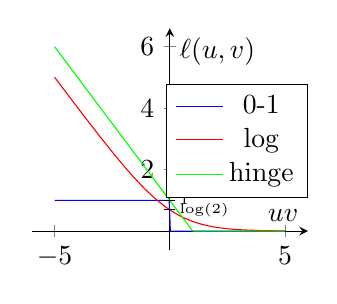
\begin{tikzpicture}[
	declare function={zerone(\x)=(1)*(\x<=0) + (0)*(\x>0);}
	]
\begin{axis}[xlabel=$uv$,ylabel={$\ell(u,v)$},axis lines=middle,enlargelimits,width=0.42\textwidth,
	legend style={at={(1,0.75)},nodes={scale=1,transform shape}}]
	\addplot[samples=200,blue] {zerone(x)};
	\addplot[samples=200,red,smooth] {ln(1+exp(-x))}; % log-loss
	\addplot[samples=200,green,smooth] {max(0,1-x)}; % hinge loss

	\addplot[black,mark=-,nodes near coords=$\log(2)$,font={\tiny},every node near coord/.style={anchor=180}] coordinates {(0,{ln(2)})};
	\addplot[black,mark=-,nodes near coords=$1$,font={\tiny},every node near coord/.style={anchor=180}] coordinates {(0,1)};

	\legend{0-1, log, hinge}
\end{axis}
\end{tikzpicture}
\caption{Loss functions}
\label{fig:losses}
\end{figure}


\subsection{Logistic regression}

Logistic regression uses the logistic function to model the probability as follows
\[
m(x)=\sigma(x)=\frac{1}{1+\exp\bigl(-(w^Tx+b)\bigr)}\rightarrow\log\biggl(\frac{m(x)}{1-m(x)}\biggr)=w^Tx+b
\]

The empirical risk minimization
\[
\min_{w,b}\frac{1}{N}\sum_{i=1}^N\log\biggl(1+\exp\Bigl(-y^{(i)}\bigl(w^Tx^{(i)}+b\bigr)\Bigr)\biggr)
\]



\section{Multi-class classification}

\subsection{Multinomial logistic regression}

































